% Perpendicular bisectors of a triangle
% Author: Sam Britt
\documentclass[tikz,border=10pt]{standalone}
%%%<
\usepackage{verbatim}
%%%>
\begin{comment}
:Title: Perpendicular bisectors of a triangle
:Tags: Coordinate calculations;Foreach;Mathematical engine;Geometry;Mathematics
:Author: Sam Britt
:Slug: bisector

A perpendicular bisector of a line segment is a line which is perpendicular
to this line and passes through its midpoint. This drawing shows
perpendicular bisectors of a triangle. They meet in the center of the
circumcircle of the triangle.

This example was written by Sam Britt answering a question on TeX.SE.
\end{comment}
\usetikzlibrary{calc}
\begin{document}
\def\centerarc[#1](#2)(#3:#4:#5)% Syntax: [draw options] (center) (initial angle:final angle:radius)
{ \draw[#1] ($(#2)+({#5*cos(#3)},{#5*sin(#3)})$) arc (#3:#4:#5); }

\begin{tikzpicture}
 [
  scale=2,
  >=stealth,
  point/.style = {draw, circle,  fill = black, inner sep = 1pt},
  dot/.style   = {draw, circle,  fill = black, inner sep = .2pt},
 ]

 % the circle
 \def\rad{1}
 \node (origin) at (0,0) [point, label = {below right:$Drone$}]{};
 \node (A) at (-1,1) [point, label = {below right:$A_0$}]{};
 \node (B) at (1,1) [point, label = {below right:$B_0$}]{};
 \node (C) at (1,-1) [point, label = {below right:$C_0$}]{};
 \node (D) at (-1,-1) [point, label = {below right:$D_0$}]{};

 \draw[dotted] (A) circle (1.2);
 \draw[dotted] (A) circle (1.6);

 \draw[dotted] (B) circle (1.2);
 \draw[dotted] (B) circle (1.6);

 \draw[dotted] (C) circle (1.2);
 \draw[dotted] (C) circle (1.6);

 \draw[dotted] (D) circle (1.2);
 \draw[dotted] (D) circle (1.6);
\end{tikzpicture}

\begin{tikzpicture}
 [
  scale=2,
  >=stealth,
  point/.style = {draw, circle,  fill = black, inner sep = 1pt},
  dot/.style   = {draw, circle,  fill = black, inner sep = .2pt},
 ]

 % the circle
 \def\rad{1}
 \node (origin) at (0,0) [point, label = {below right:$Drone$}]{};
 \node (A) at (-1,1) [point, label = {below right:$A_0$}]{};
 \node (B) at (1,1) [point, label = {below right:$B_0$}]{};
 \node (C) at (1,-1) [point, label = {below right:$C_0$}]{};
 \node (D) at (-1,-1) [point, label = {below right:$D_0$}]{};

 \draw[dotted] (A) circle (1.2);
 \draw[dotted] (A) circle (1.6);

 \draw[dotted] (B) circle (1.2);
 \draw[dotted] (B) circle (1.6);

 \draw[dotted] (C) circle (1.2);
 \draw[dotted] (C) circle (1.6);

 \draw[dotted] (D) circle (1.2);
 \draw[dotted] (D) circle (1.6);
\end{tikzpicture}

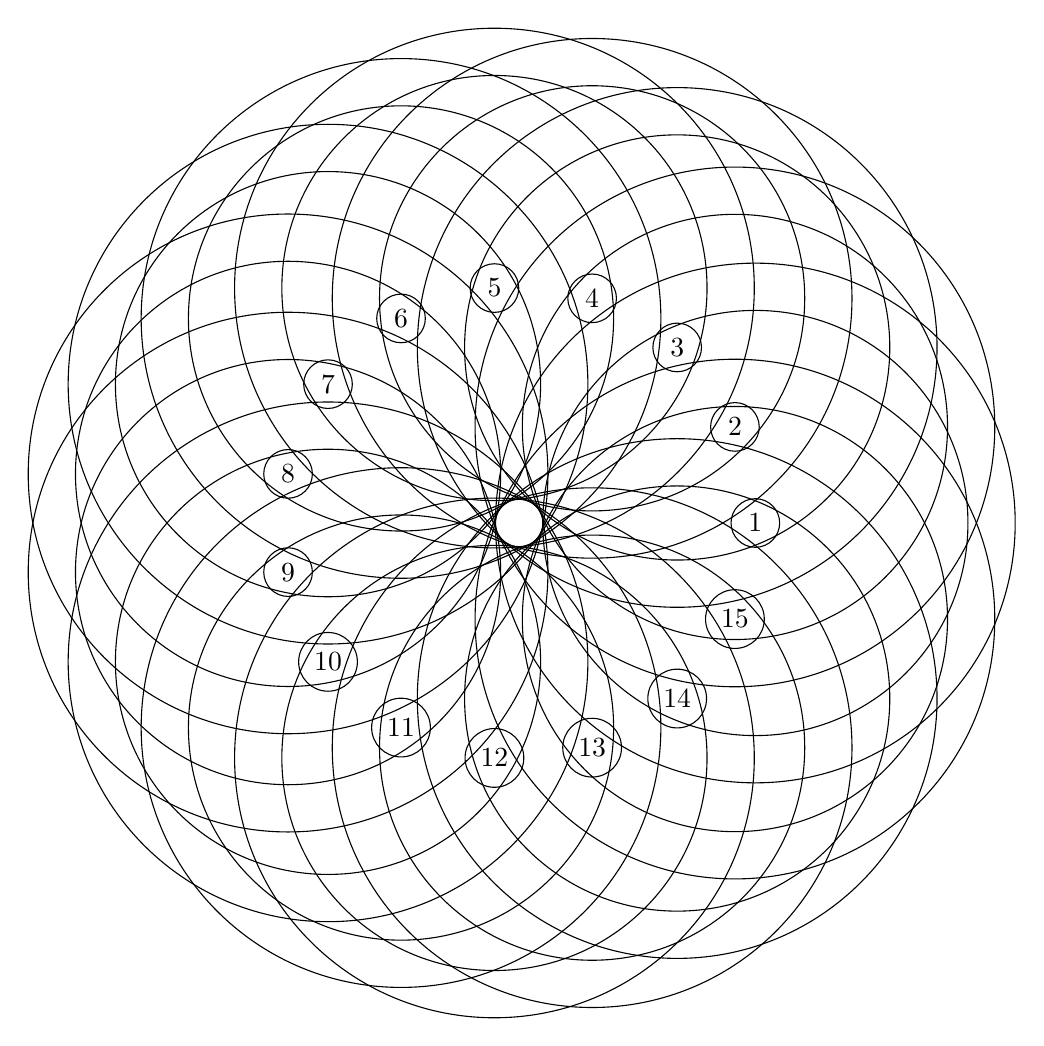
\begin{tikzpicture}
 [
  scale=3,
  >=stealth,
  point/.style = {draw, circle,  fill = black, inner sep = 1pt},
  dot/.style   = {draw, circle,  fill = black, inner sep = .2pt},
 ]
 \def \n {15}
 \def \radius {1}
 \def \margin {8} % margin in angles, depends on the radius
 \def\rad{1}
 \def\error{0.1}

 \foreach \s in {1,...,\n}
 {
  \node[draw,circle] (\s) at ({360/\n * (\s - 1)}:\radius) {$\s$};
  \draw (\s) circle (\rad+\error);
  \draw (\s) circle (\rad-\error);
  % \draw[->, >=latex] ({360/\n * (\s - 1)+\margin}:\radius)
  % arc ({360/\n * (\s - 1)+\margin}:{360/\n * (\s)-\margin}:\radius);
 }
\end{tikzpicture}
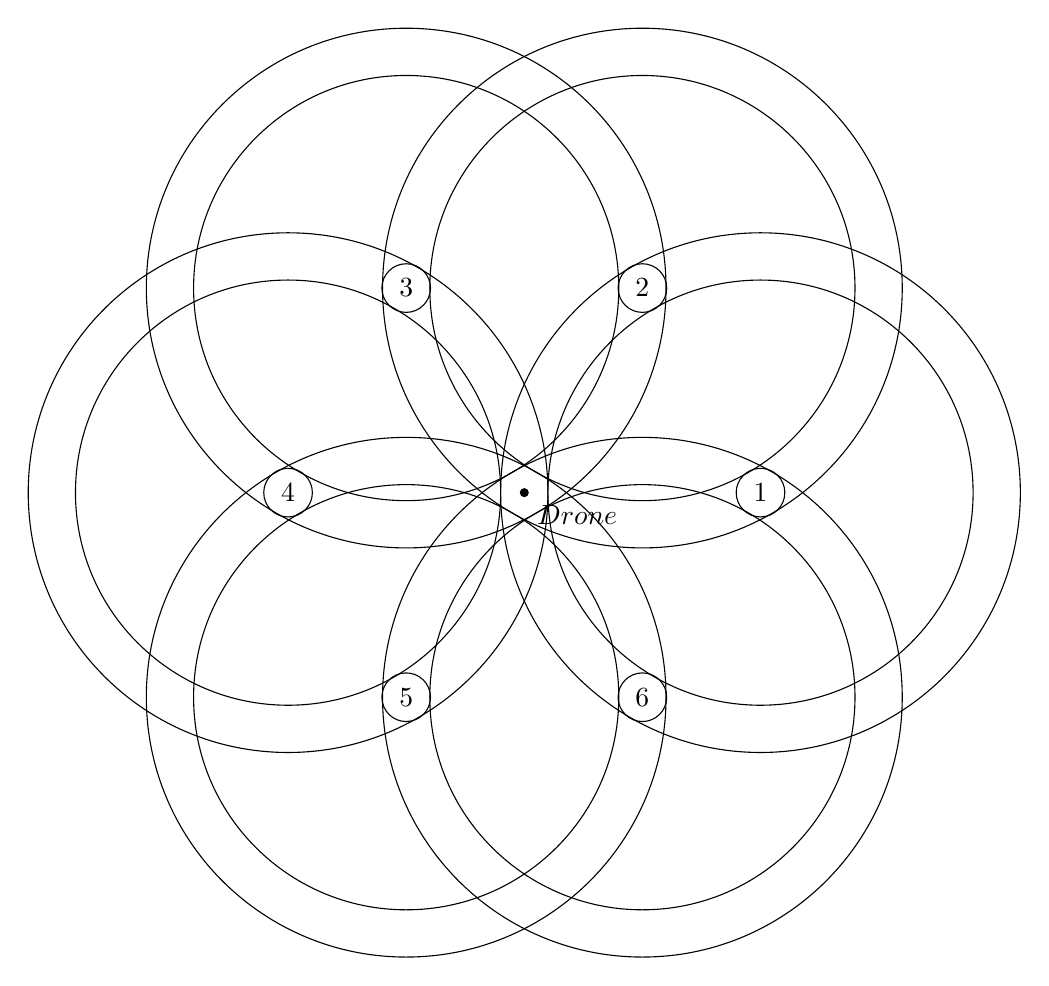
\begin{tikzpicture}
 [
  scale=3,
  >=stealth,
  point/.style = {draw, circle,  fill = black, inner sep = 1pt},
  dot/.style   = {draw, circle,  fill = black, inner sep = .2pt},
 ]
 \def \n {6}
 \def \radius {1}
 \def \margin {8} % margin in angles, depends on the radius
 \def\rad{1}
 \def\error{0.1}
 \node (origin) at (0,0) [point, label = {below right:$Drone$}]{};
 \foreach \s in {1,...,\n}
 {
  \node[draw,circle] (\s) at ({360/\n * (\s - 1)}:\radius) {$\s$};
  \draw (\s) circle (\rad+\error);
  \draw (\s) circle (\rad-\error);
  \centerarc[red,thick] (\s) (0:90:1)
  % \draw[->, >=latex] ({360/\n * (\s - 1)+\margin}:\radius)
  % arc ({360/\n * (\s - 1)+\margin}:{360/\n * (\s)-\margin}:\radius);
 }
\end{tikzpicture}
\end{document}
